\chapter{Projekt, architektura aplikacji i jej zastosowanie}
\section{Wprowadzenie}
W celu dopasowania oprogramowania do założeń przedstawionych w poprzednim rozdziale, do realizacji wybrano narzędzia pozwalające na bezbolesną integrację, możliwie najniższe wymagania sprzętowe, niską ilość zależności (ang. dependencies) oraz przejrzystość kodu źródłowego. W tym rozdziale przedstawiona zostanie ogólna architektura rozwiązania, jego elementy.

\section{Architektura rozwiązania}
Ogólną strukturę aplikacji oraz komunikację pomiędzy jej najważniejszymi elementami przedstawiono na rysunku \ref{fig:application_architecture}:

\begin{figure}[H]
    \centering
    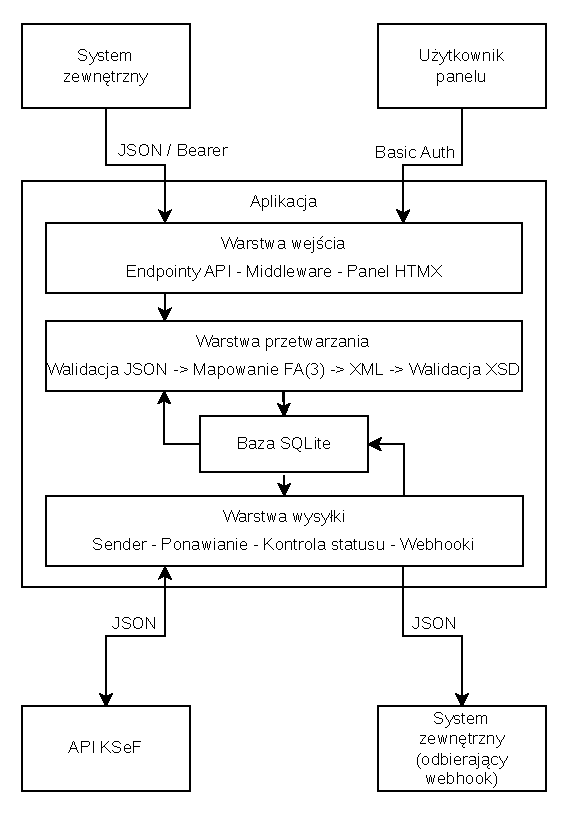
\includegraphics[width=\textwidth]{images/app_layers.pdf}
    \caption{Architektura aplikacji integracyjnej}
    \label{fig:application_architecture}
\end{figure}

\subsection{Warstwa wejścia}
Składa się z kolejnych endpointów serwera HTTP, przyjmujących żądania od zewnętrznych systemów w postaci JSON, lub żądań od przeglądarki, zwracając HTML lub odpowiednie triggery HTMX. Endpointy podzielone są na dwie kategorie - te odpowiedzialne za przyjmowanie faktur oraz zapytań z nimi związanych oraz obsługujące interfejs panelu użytkownika. Dane przyjęte w tej warstwie przekazywane są głębiej do aplikacji. Zwracane są ustrukturyzowane odpowiedzi w formacie JSON.

\subsection{Warstwa przetwarzania danych}
Przyjęte dane są procesowane poprzez sprawdzenie elementów faktury pod kątem poprawności. Otrzymany JSON transformowany jest w czyste obiekty w języku Go, po czym transformowany w format XML. Walidator, utworzony przy uruchomieniu programu, sprawdza strukturę wygenerowanych danych, porównując ją do oficjalnego schematu XSD. Z pełnego kompletu wymaganych elementów tworzony jest obiekt odpowiadający rekordowi w bazie danych.

\subsection{Warstwa przechowywania danych}
Dane przechowywane są w relacyjnej bazie danych SQLite. Rozwiązanie to zostało wybrane ze względu na swoją prostotę w porównaniu do innych podobnych technologii (takich jak przykładowo PostgreSQL) oraz lokalne przechowywanie danych. Warstwa ta odpowiedzialna jest za odpowiedni zapis przyjmowanych faktur oraz ich obecnego stanu, korzystając z odpowiednich kolumn pozwalających innym elementom aplikacji wykonywać adekwatne działania na rekordach. Istnieje tylko pojedyncza tabela - \texttt{Invoices} (pol. Faktury) - która przechowuje następujące dane: 

\begin{small}
\begin{longtable}{>{\raggedright\arraybackslash}p{4cm} >{\raggedright\arraybackslash}p{2cm} >{\raggedright\arraybackslash}p{7cm}}
    \caption{Najważniejsze kolumny tabeli \texttt{Invoices} w lokalnej bazie danych}
\label{tab:sqlite_invoices} \\
\toprule
\textbf{Kolumna} & \textbf{Typ} & \textbf{Opis} \\
\midrule
\endfirsthead

\toprule
\textbf{Kolumna} & \textbf{Typ} & \textbf{Opis} \\
\midrule
\endhead

\bottomrule
\endfoot

id & INTEGER & Klucz główny rekordu. \\
external\_id & TEXT & Numer faktury w systemie zewnętrznym. \\
raw\_json & TEXT & Oryginalne dane otrzymane w formacie JSON. \\
raw\_xml & TEXT & Faktura przekonwertowana do formatu XML. \\
status & TEXT & Status przetwarzania faktury - \texttt{PENDING}, \texttt{PROCESSING}, \texttt{SENT}, \texttt{FAILED} lub \texttt{UNKNOWN}. \\
ksef\_id & TEXT & Numer faktury w KSeF. \\
ksef\_error & TEXT & Błąd zwrócony przez KSeF w przypadku odrzucenia. \\
upo\_xml & TEXT & Urzędowe Poświadczenie Odbioru w formacie XML. \\
attempt\_count & INTEGER & Liczba prób ponownych wysłania faktury do KSeF. \\
created\_at & DATETIME & Data utworzenia. \\
updated\_at & DATETIME & Data ostatniej aktualizacji. \\
submission\_reference & TEXT & Identyfikator przesłania, nadany przez KSeF. \\
callback\_url & TEXT & Opcjonalny adres do przesłania informacji dotyczącej statusu faktury, po zakończeniu przetwarzania. \\
webhook\_delivered & BINARY & Informacja, czy dane dotyczące statusu przesyłki zostały zwrócone. \\
webhook\_attempt\_count & INTEGER & Liczba prób ponownych dostarczenia informacji zwrotnej. \\
webhook\_error & TEXT & Błąd w przypadku niepomyślnego dostarczenia informacji zwrotnej. \\
\end{longtable}
\end{small}

Kolumna \texttt{status} pozwala na pięć różnych wartości:
\begin{small}
\begin{longtable}{>{\raggedright\arraybackslash}p{3cm} >{\raggedright\arraybackslash}p{10cm}}
\caption{Wartości kolumny \texttt{status} w tabeli \texttt{Invoices}}
\label{tab:invoice_statuses} \\
\toprule
\textbf{Status} & \textbf{Znaczenie} \\
\midrule
\endfirsthead

\toprule
\textbf{Status} & \textbf{Znaczenie} \\
\midrule
\endhead

\bottomrule
\endfoot

\texttt{PENDING} & Faktura została przyjęta przez aplikację i oczekuje na przetwarzanie oraz próbę wysyłki. \\
\texttt{PROCESSING} & Faktura została pobrana przez mechanizm wysyłki i obecnie jest w trakcie przetwarzania. Zależnie od efektu końcowego podejmowanych prób, status zostanie zmieniony. \\
\texttt{SENT} & Faktura została wysłana do Krajowego Systemu e-Faktur, a aplikacja otrzymała Urzędowe Poświadczenie Odbioru. \\
\texttt{FAILED} & Faktura nie mogła zostać wysłana, lub została odrzucona przez Krajowy System e-Faktur. Podjęta została maksymalna liczba prób ponownych wysyłki. \\
\texttt{UNKNOWN} & Faktura została wysłana, ale nie otrzymano informacji zwrotnej z Krajowego Systemu e-Faktur. W trakcie kolejnych cykli działania aplikacji podjęte zostaną próby uzyskania odpowiedzi dotyczącej stanu faktury, by przypisać jej odpowiedni status. \\
\end{longtable}
\end{small}

W przypadku przyjęcia faktury o zewnętrznym identyfikatorze identycznym do faktury już istniejącej w bazie danych, o statusie \texttt{FAILED}, rekord zostanie nadpisany, traktując nowe żądanie jako poprawioną wersję poprzedniej.

\subsection{Warstwa przetwarzania w tle}
Warstwa ta składa się z cyklicznego mechanizmu, który skanuje bazę danych w poszukiwaniu rekordów wymagających przetwarzania, zależnie od ich statusu. Mechanizm ten pobiera zbiór faktur (z limitem określanym przez użytkownika w pliku konfiguracyjnym), następnie uruchamia asynchroniczne procesy wysyłki dla każdego z nich. Faktury oraz webhooki, których wysyłka się nie powiodła, ale nie osiągnęły limitu prób ponownych wysyłki, również są procesowane w kolejnych cyklach. Pobierane są również faktury o statusie \texttt{UNKNOWN} w celu sprawdzenia ich statusu.

\subsection{Warstwa integracji z systemami zewnętrznymi}
Warstwa ta odpowiada za komunikację z Krajowym Systemem e-Faktur, oraz systemami, od których aplikacja przyjmuje faktury. Autentykuje użytkownika na podstawie tokenu wprowadzonego w pliku ze zmiennymi środowiskowymi, odświeża pozyskany token pozwalający na wysyłkę w przypadku jego przedawnienia, otwiera i zamyka sesje interaktywne w celu wysyłki, sprawdza ich status oraz pobiera Urzędowe Poświadczenia Odbioru. Cała komunikacja odbywa się poprzez wysyłanie żądań w HTTP oraz przyjmowanie odpowiedzi w odpowiednich formatach opisanych przez oficjalną dokumentację Krajowego Systemu e-Faktur. 

Komunikacja odbywa się również z systemami, które wysyłając aplikacji fakturę, przesłały adres URL, na który wysłana ma zostać informacja zwrotna. Warstwa wysyła odpowiednio ustrukturyzowane żądania w formacie JSON zawierające informacje dotyczące statusu końcowego (\texttt{SENT} lub \texttt{FAILED}) faktur, które zostały przetworzone.

\subsection{Warstwa wizualna oraz kontroli}
Aplikacja eksponuje panel wizualny dla użytkownika, w postaci listy rekordów z bazy danych. Użytkownik może filtrować listę przez status faktury, oraz wyszukiwać je za pomocą ich zewnętrznego identyfikatora. Możliwy jest również szczegółowy podgląd pojedynczej faktury oraz manualne jej usunięcie, jeśli jest o statusie \texttt{FAILED}. W przypadku, gdy wysyłki webhooka osiągnęły swój limit prób ponownych, możliwy jest również manualny reset licznika za pomocą przycisku. Panel jest automatycznie i dynamicznie odświeżany, bez przeładowywania strony.  

\subsection{Warstwa bezpieczeństwa}
Dane uwierzytelniające i poufne wymagane do działania aplikacji pobierane są ze zmiennych środowiskowych. \texttt{APP\_API\_KEY} to klucz, który musi być załączany do żądań przesyłanych przez systemy zewnętrzne na endpointy służące do komunikacji z nimi, w nagłówku \texttt{Authorization} w schemacie \texttt{Bearer}. \texttt{DASHBOARD\_USERNAME} oraz \texttt{DASHBOARD\_PASSWORD} chronią endpointy odpowiedzialne za interfejs i służą do uwierzytelnienia użytkownika przy próbie dostępu do wspomnianego w poprzedniej subsekcji panelu wizualnego, za pomocą HTTP Basic Authentication (przypis). Niepowodzenie w uwierzytelnieniu w czasie interakcji z endpointami jego wymagającymi skutkuje odpowiedzią o kodzie HTTP 401, \enquote{Unauthorized}. \texttt{KSEF\_TOKEN} to token uwierzytelniający, pobierany przez użytkownika z Panelu Podatnika Krajowego Systemu e-Faktur i umożliwia komunikację z samym KSeF.

\section{Przepływ przetwarzania faktury}
Możliwe zmiany statusu faktury podczas jej przetwarzania przedstawiono na rysunku \ref{fig:invoice_state_transitions}.

\begin{figure}[H]
    \centering
    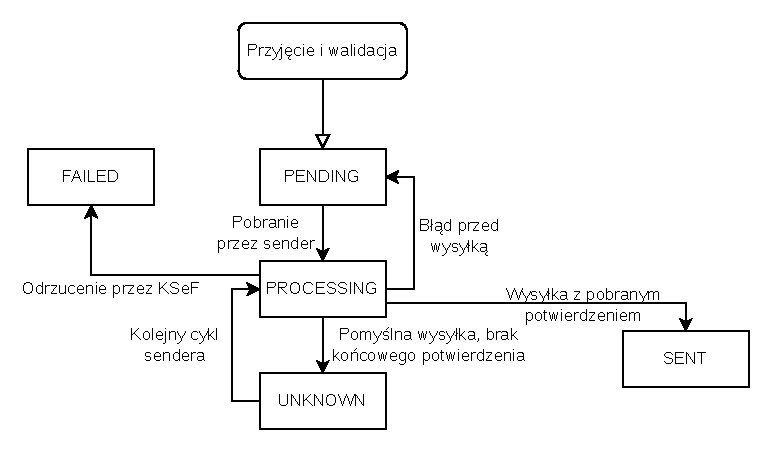
\includegraphics[width=\textwidth]{images/invoice_states.pdf}
    \caption{Przejścia pomiędzy stanami przetwarzania faktury}
    \label{fig:invoice_state_transitions}
\end{figure}

\subsection{Wejście}
Proces rozpoczyna się poprzez przyjęcie danych w formacie JSON od systemu zewnętrznego poprzez żądanie POST do endpointu \texttt{/invoices}, eksponowanego przez aplikację. 
Format JSON został wybrany ze względu na swoją kompatybilność z HTTP API oraz szerokie wsparcie przez systemy zintegrowane i aplikacje backendowe. Jest on również czytelny dla człowieka. Aplikacja akceptuje dane w formacie JSON, służącym jako pośredni, integracyjny format, i używa ich do stworzenia bardziej ustrukturyzowanego pliku XML dostosowanego do oficjalnego schematu (FA3) udostępnionego przez Ministerstwo Finansów
% citation
. 

\noindent Oprogramowanie spodziewa się następujących danych:
\begin{small}
\begin{longtable}{>{\raggedright\arraybackslash}p{4cm} >{\raggedright\arraybackslash}p{2cm} >{\raggedright\arraybackslash}p{7cm}}
\caption{Pola żądania wejściowego HTTP przekazywanego do endpointu \texttt{/invoices}}
\label{tab:invoice_input_fields} \\
\toprule
\textbf{Pole} & \textbf{Wymagalność} & \textbf{Opis} \\
\midrule
\endfirsthead

\toprule
\textbf{Pole} & \textbf{Wymagalność} & \textbf{Opis} \\
\midrule
\endhead

\bottomrule
\endfoot

invoice\_type & TAK & Typ faktury - VAT, korygująca, zaliczkowa, rozliczeniowa, uproszczona, korygująca rozliczeniowa lub korygująca zaliczkowa. \\
invoice\_number & TAK & Numer faktury w systemie zewnętrznym. \\
issue\_date & TAK & Data wystawienia faktury w formacie RRRR-MM-DD. \\
currency & TAK & Kod waluty zgodny z ISO 4217. \\
exchange\_rate & TAK / NIE & Kurs waluty dla walut innych niż PLN. \\
total\_amount & TAK & Łączna wartość brutto faktury. \\
seller & TAK & Dane sprzedawcy - NIP, nazwa oraz adres. \\
buyer & TAK & Dane nabywcy - w przypadku faktury uproszczonej wymagany jest jedynie NIP. \\
items & TAK & Lista wierszy faktury, zawierająca nazwę, ilość, wartość netto oraz stawkę podatku dla każdej usługi/produktu. \\
tax\_breakdowns & TAK & Wartości netto i podatku, podzielone przez stawki VAT. \\
payment & NIE & Dane dotyczące płatności - termin płatności, metoda i rachunek bankowy. \\
flags & NIE & Dodatkowe znaczniki, przykładowo płatność podzielona lub metoda kasowa. \\
callback\_url & NIE & Adres URL, na który oprogramowanie wyśle informację o statusie przesyłki. \\
original\_invoice\_number & NIE & Numer oryginalnej faktury, wymagany w przypadku faktur korygujących. \\
original\_issue\_date & NIE & Data wystawienia oryginalnej faktury, wymagana w przypadku faktur korygujących. \\
original\_ksef\_id & NIE & Numer identyfikacyjny faktury w KSeF, wymagany w przypadku faktur korygujących. \\
correction\_reason & NIE & Powód korekty, wymagany w przypadku faktur korygujących. \\
corrected\_buyer & TAK / NIE & Poprawione dane nabywcy, wymagane w przypadku faktur korygujących. \\
\end{longtable}
\end{small}

\subsection{Walidacja otrzymanych danych}
Faktura jest następnie przetwarzana - występuje walidacja podstawowych danych faktury w celu stwierdzenia, czy powinna zostać podjęta próba przesłania jej do Krajowego Systemu e-Faktur. Sprawdzane dane to:
\begin{itemize}
    \item Typ faktury - faktura VAT, faktura korygująca, faktura zaliczkowa, faktura rozliczeniowa, faktura uproszczona, faktura korygująca rozliczeniowa lub faktura korygująca zaliczkowa.
    \item W przypadku faktur korygujących, sprawdzane są pola dotyczące danych korekty - powód, data wystawienia oryginalnej faktury, poprawność daty oraz poprawione dane kontrahenta. W przypadku faktur niekorygujących, pola sprawdzane są z założeniem, że powinny być puste.
    \item Podstawowa walidacja waluty - ilość znaków, oraz w przypadku walut innych niż PLN, kurs między określoną walutą a PLN. 
    \item Wiersze sprzedaży - aplikacja sprawdza, czy faktura nie jest pusta. Następnie waliduje każdy wiersz sprzedaży, poprzez sprwadzenie ilości określonego produktu/usługi, ceny na jednostkę oraz nałożenia odpowiedniego podatku. W przypadku faktur niekorygujących, odrzuca wartości netto poniżej zera. Wartości netto oraz podatku są zsumowane i walidowane przeciwko całkowitej wartości faktury.
    \item Dane kontrahentów - sprawdzane są Numery Identyfikacji Podatkowej obu stron wykonanej transakcji poprzez sprawdzenie ich odpowiednim algorytmem oraz nazwy i adresy stron. Walidowany jest również kod kraju sprzedawcy, a w przypadku jego braku, następuje wprowadzenie wartości domyślnej - PL. W przypadku faktury uproszczonej, dane kupującego, poza Numerem Identyfikacji Podatkowej, nie są wymagane % przypis.
\end{itemize}

\subsection{Utworzenie pliku w formacie XML}
Dane są następnie transformowane do formatu XML wymaganego przez Krajowy System e-Faktur, poprzez mapowanie odpowiednich pól JSON do pól wymaganych przez oficjalny schemat XSD, m.in. nagłówek, informacje dotyczące sprzedawcy oraz nabywcy, wiersze sprzedaży, wartości podatkowe, informacje o płatności oraz ewentualnie pola korygujące.
Pola są generowane na podstawie struktur odpowiadających elementom końcowego pliku XML, a nie korzystając z manipulacji tekstem, minimalizując prawdopodobieństwo niepoprawności dokumentu. 

\subsection{Walidacja danych w formacie XML}
Aplikacja waliduje nowo utworzone dane XML wobec schematu XSD udostępnionego przez Ministerstwo Finansów, sprawdzając poprawność pól pod względem typów i dopuszczalnych wartości oraz strukturę dokumentu - kolejność, odpowiednie zagnieżdżenie elementów.

\subsection{Zapis danych}
W przypadku pomyślności poprzednich kroków, dane zapisywane są w lokalnej bazie danych SQLite, najpierw sprawdzając, czy identyfikator nadany jej przez zewnętrzny system już w niej występuje. Jeśli tak, a poprzednio zapisany rekord nie został poprawnie przesłany do Krajowego Systemu e-Faktur, aplikacja zastępuje ją, traktując nowe żądanie jako korektę poprzedniej faktury.

Tabela przedstawiająca strukturę rekordów przechowywanych w bazie danych została przedstawiona w tabeli \ref{tab:sqlite_invoices}.

\subsection{Lokalna kolejka oraz wysyłka}
Aplikacja skanuje bazę danych w poszukiwaniu faktur oznaczonych jako niewysłane oraz dodaje je do lokalnej kolejki. Jeśli kolejka nie jest pusta, otwierana jest sesja interaktywna przez uwierzytelnienie w KSeF, faktury są wysyłane oraz monitorowane pod względem statusu wysyłki. W przypadku akceptacji, faktura oznaczana jest jako wysłana - w przypadku nieznanego statusu, aplikacja ponowi zapytanie dotyczące faktury. Jeśli zaś dojdzie do porażki, aplikacja spróbuje wysłać fakturę ponownie w następnym cyklu działania, do momentu gdy nie zostanie osiągnięty określony przez użytkownika w pliku konfiguracyjnym limit prób ponownych. Wyjątkiem jest tutaj błąd połączenia z internetem - w tym wypadku, faktura pozostanie w kolejce, do momentu, gdy możliwa będzie wysyłka.

\subsection{Webhooki}
Jeśli w oryginalnych danych przekazanych aplikacji żądaniem figurował adres, na który wysłana powinna zostać informacja zwrotna dotycząca statusu wysyłki, mechanizm webhooków (\textit{webhook} - dosł. hak sieciowy - aplikacja zapamiętuje dostawcę danych, na potrzebę przyszłej interakcji)
prześle zewnętrznemu systemowi dane w formacie JSON po oznaczeniu faktury jako wysłana lub odrzucona, potwierdzając pomyślność operacji lub podając powód odrzucenia faktury. W przypadku błędu w trakcie próby przekazania danych, aplikacja podejmie kolejne próby, aż do osiągnięcia określonego przez użytkownika limitu prób ponownych. Zresetowanie licznika prób ponownych może zostać wykonane przez użytkownika z poziomu panelu dostępnego przez przeglądarkę.

\noindent Informacja zwrotna przesyłana jest w następującej postaci:
\begin{small}
\begin{longtable}{>{\raggedright\arraybackslash}p{4cm} >{\raggedright\arraybackslash}p{2cm} >{\raggedright\arraybackslash}p{7cm}}
\caption{Pola żądania HTTP z informacją zwrotną przesyłanego do systemu zewnętrznego}
\label{tab:webhook_payload} \\
\toprule
\textbf{Pole} & \textbf{Typ} & \textbf{Opis} \\
\midrule
\endfirsthead

\toprule
\textbf{Pole} & \textbf{Typ} & \textbf{Opis} \\
\midrule
\endhead

\bottomrule
\endfoot

event & TEXT & Typ zdarzenia, przykładowo invoice.accepted lub invoice.failed. \\
invoice\_id & INTEGER & Identyfikator faktury w aplikacji - klucz główny w bazie danych. \\
external\_id & TEXT & Numer faktury pochodzący z systemu zewnętrznego. \\
status & TEXT & Status wysyłki - \texttt{SENT} lub \texttt{FAILED}. \\
ksef\_reference\_number & TEXT / NULL & Numer faktury w KSeF, jeśli faktura została przyjęta. \\
submission\_reference & TEXT / NULL & Identyfikator przesłania, nadany przez KSeF. \\
error\_message & TEXT / NULL & Błąd, który nastąpił w przypadku niepowodzenia. \\
timestamp & DATETIME & Czas przesyłki informacji zwrotnej. \\
\end{longtable}
\end{small}

\subsection{Panel użytkownika}
Aplikacja eksponuje również prosty panel na endpoincie \texttt{/ui/invoices} umożliwiający wgląd do historii wysyłek, filtrowanie faktur według statusu, wyszukiwanie pojedynczych rekordów oraz ich manualne usuwanie w przypadku niepomyślnej wysyłki i osiągnięcia limitu prób ponownych. Możliwy jest również reset licznika prób ponownych wysyłki webhooków, jeśli limit został poprzednio osiągnięty. Panel automatycznie odświeża swoją zawartość. Panel wykonany został z użyciem HTMX oraz ostylowany za pomocą Tailwind CSS.

\section{Komunikacja z KSeF}
Podstawowym elementem działania aplikacji jest interakcja z samym Krajowym Systemem e-Faktur - uwierzytelnienie, otwieranie i zamykanie sesji interaktywnych w celu wysyłki faktur oraz sprawdzanie statusu i odbiór Urzędowych Poświadczeń Odbioru. 

\subsection{Uwierzytelnienie}
Uwierzytelnienie następuje natychmiast po uruchomieniu aplikacji i podtrzymywane jest przez cały okres jej działania. Aplikacja wykonuje puste żądanie POST do endpointu \texttt{/auth/challenge} eksponowanego przez KSeF, w odpowiedzi uzyskując \enquote{wyzwanie} - timestamp, który po połączeniu z pozyskanym wcześniej przez użytkownika tokenem API z panelu KSeF jest szyfrowany z użyciem klucza publicznego automatycznie pobieranego przez aplikację. Przesyłane następnie jest żądanie do endpointu \texttt{/auth/ksef-token}, zwracające tymczasowy token dostępu. Następnie, token ten wysyłany jest do \texttt{/auth/token/redeem}, pozyskując token dostępu oraz drugi, pozwalający na odświeżenie go. Oprogramowanie automatycznie sprawdza, kiedy dojdzie do przedawnienia, i automatycznie odświeży status uwierzytelnienia, jeśli jest taka potrzeba.

\subsection{Otwieranie i zamykanie sesji}
Do otwierania oraz zamykania tzw. sesji interaktywnych, pozwalających na wysyłkę faktur, dochodzi gdy aplikacja rejestruje pojawienie się nowej faktury lub faktur do wysyłki w bazie danych. Sesja otwierana jest poprzez przesłanie żądania z zaszyfrowanym kluczem symetrycznym oraz wektorem inicjalizacji do endpointu \texttt{/sessions/online}, otrzymując w odpowiedzi identyfikator sesji oraz czas jej ważności. Po wysyłce sesja jest zamykana przez przesłanie żądania do endpointu \texttt{/sessions/online/x/close}, gdzie \enquote{x} jest zapisanym przy otwarciu identyfikatorem.

\subsection{Przesyłanie faktur}
Faktury z bazy danych, w formacie XML, są następnie szyfrowane oraz przesyłane do endpointu \texttt{/sessions/online/x/invoices}, gdzie \enquote{x} to identyfikator sesji interaktywnej. Zwracany jest identyfikator przesyłki, który wykorzystywany jest do sprawdzenia statusu wysyłki. Niepotwierdzane jest jednak czy faktura została przyjęta przez KSeF.

\subsection{Sprawdzenie statusu i pobranie Urzędowego Poświadczenia Odbioru}
Aplikacja sprawdza status faktury aż do otrzymania odpowiedzi, lub osiągnięcia limitu ponownych żądań ustalonego przez użytkownika w konfiguracji. W przypadku przyjęcia faktury przez KSeF, aplikacja zapisze Urzędowe Poświadczenie Odbioru w bazie danych, a w przypadku odrzucenia oznaczy w bazie danych porażkę. W przypadku otrzymywania odpowiedzi, że faktura dalej jest przetwarzana, oznaczy jej status jako nieznany, oraz podejmie próbę sprawdzenia jej statusu przy kolejnym cyklu kolejki.

\section{Cykl życia aplikacji}
W tej sekcji opisane będzie ogólne działanie - od konfiguracji i uruchomienia, przez działanie, po mechanizm bezpiecznego zamknięcia oraz w jaki sposób aplikacja jest wdrażana kontenerowo.

\subsection{Konfiguracja}
Oprogramowanie jest konfigurowane za pomocą pliku \texttt{config.yaml}, którego format został wybrany ze względu na swoją prostotę, czytelność dla człowieka oraz powielenie użycia we wdrożeniu kontenerowym (plik \texttt{docker-compose.yaml}), któremu dedykowana jest osobna subsekcja. 


\noindent Struktura pliku konfiguracyjnego jest następująca:

\begin{small}
\begin{longtable}{>{\raggedright\arraybackslash}p{4.8cm} >{\raggedright\arraybackslash}p{1.7cm} >{\raggedright\arraybackslash}p{6.5cm}}
\caption{Plik konfiguracyjny aplikacji}
\label{tab:config_fields} \\
\toprule
\textbf{Parametr} & \textbf{Typ} & \textbf{Opis} \\
\midrule
\endfirsthead

\toprule
\textbf{Parametr} & \textbf{Typ} & \textbf{Opis} \\
\midrule
\endhead

\bottomrule
\endfoot

ksef.nip & TEXT & Numer Identyfikacji Podatkowej podmiotu, który reprezentuje użytkownik. \\
ksef.url & TEXT & Oficjalny adres API KSeF, na wypadek zmiany, lub chęci użytkownika do przetestowania oprogramowania na środowisku testowym. \\
ksef.http\_timeout\_sec & INTEGER & Maksymalny czas oczekiwania na odpowiedź HTTP z KSeF. \\
ksef.auth\_retry\_delay\_sec & INTEGER & Przerwa w sekundach pomiędzy kolejnymi próbami uwierzytelnienia w KSeF. \\
ksef.polling\_delay\_sec & INTEGER & Przerwa w sekundach pomiędzy kolejnymi zapytaniami o status wysłanej do KSeF faktury. \\
ksef.confirmation\_max\_attempts & INTEGER & Maksymalna liczba prób sprawdzenia statusu przesłanej faktury. \\
sqlite.db\_path & TEXT & Ścieżka do lokalnej bazy danych, wybierana przez użytkownika. \\
sqlite.busy\_timeout\_ms & INTEGER & Czas oczekiwania SQLite na zwolnienie blokady bazy danych. \\
server.port & TEXT & Port HTTP/HTTPS, na którym uruchamiana jest aplikacja. \\
server.tls\_cert\_path & TEXT & Ścieżka do certyfikatu TLS wykorzystywanego przez serwer HTTPS. \\
server.tls\_key\_path & TEXT & Ścieżka do klucza prywatnego TLS wykorzystywanego przez serwer HTTPS. \\
user.max\_retries & INTEGER & Maksymalna liczba prób ponownych wysyłki faktury lub webhooka w przypadku błędów. \\
dash\_page\_size & INTEGER & Liczba faktur wyświetlanych na jednej stronie panelu użytkownika. \\
polling\_interval & INTEGER & Czas w sekundach między skanowaniem bazy danych w poszukiwaniu faktur do wysyłki. \\
shutdown\_timeout\_sec & INTEGER & Maksymalny czas oczekiwania na bezpieczne zamknięcie aplikacji. \\
sender\_batch\_size & INTEGER & Maksymalna liczba faktur lub webhooków wysyłanych w jednym cyklu działania aplikacji. \\
sender\_worker\_limit & INTEGER & Limit równoległych wysyłek faktur lub webhooków wykonywanych naraz przez aplikację. \\
\end{longtable}
\end{small}

Dodatkowo, użytkownik musi skonfigurować plik \texttt{.env} zawierający zmienne środowiskowe, poprzez skopiowanie, zmianę nazwy i uzupełnienie pliku \texttt{.env.example}. Te zmienne występują w osobnym pliku, ponieważ wszystkie poza \texttt{DASHBOARD\_USERNAME} są danymi poufnymi - ich jawność mogłaby umożliwić dostęp do aplikacji osobom trzecim. 

\begin{small}
\begin{longtable}{
    >{\raggedright\arraybackslash}p{5.2cm}
    >{\raggedright\arraybackslash}p{9cm}
}
\caption{Zmienne środowiskowe wymagane przez aplikację}
\label{tab:environment_variables} \\
\toprule
\textbf{Zmienna} & \textbf{Opis} \\
\midrule
\endfirsthead

\toprule
\textbf{Zmienna} & \textbf{Opis} \\
\midrule
\endhead

\bottomrule
\endfoot

KSEF\_TOKEN
& Token uwierzytelniający uzyskany przez użytkownika z Krajowego Systemu e-Faktur. \\

APP\_API\_KEY
& Klucz wykorzystywany do uwierzytelniania systemów zewnętrznych korzystających z endpointów API aplikacji. \\

DASHBOARD\_USERNAME
& Nazwa użytkownika wymagana podczas uwierzytelniania w panelu użytkownika. \\

DASHBOARD\_PASSWORD
& Hasło wymagane podczas uwierzytelniania w panelu użytkownika. \\

\end{longtable}
\end{small}

Brak wartości w którymkolwiek z pól nie pozwoli użytkownikowi na uruchomienie aplikacji.

\subsection{Uruchomienie aplikacji}
Po uruchomieniu aplikacji, tworzone są loggery odpowiadające za rejestrowanie wszystkich działań aplikacji. Otwierany jest wcześniej wspomniany plik konfiguracyjny, a jego wartości są walidowane. Wczytywane są również zmienne środowiskowe. Oprogramowanie utworzy odpowiednią bazę danych SQLite, lub spróbuje połączyć się z już isntiejącą, jeśli owa istnieje. Następnie tworzony jest specjalny walidator wykorzystujący oficjalny schemat XSD FA(3) do sprawdzenia poprawności strukturalnej faktur. 

Tworzony jest klient HTTP oraz struktura aplikacji, z użyciem parametrów z pliku konfiguracyjnego, oraz uruchamiany jest serwer HTTP lub HTTPS (zależnie od tego, czy użytkownik dostarczył certyfikat oraz klucz TLS), asynchronicznie z pętlą odpowiadającą za skanowanie bazy danych w poszukiwaniu faktur. Przygotowywany jest również kontekst pozwalający później na bezpieczne zamknięcie aplikacji. 

\subsection{Działanie aplikacji}
Aplikacja w ramach swojego działania eksponuje odpowiednie endpointy API HTTP oraz rozpoczyna cykliczne skanowanie bazy danych SQLite. Endpointy służące do komunikacji z zewnętrznymi systemami zwracają ustrukturyzowane odpowiedzi w formacie JSON, a endpointy wspomagające panel użytkownika przekazują HTML lub odpowiedzi specyficzne do HTMX.

\noindent Eksponowane są następujące endpointy:

\begin{small}
\begin{longtable}{>{\raggedright\arraybackslash}p{1.7cm} >{\raggedright\arraybackslash}p{4.3cm} >{\raggedright\arraybackslash}p{2.0cm} >{\raggedright\arraybackslash}p{4.6cm}}
\caption{Endpointy eksponowane przez aplikację}
\label{tab:app_endpoints} \\
\toprule
\textbf{Metoda} & \textbf{Endpoint} & \textbf{Dostęp} & \textbf{Opis} \\
\midrule
\endfirsthead

\toprule
\textbf{Metoda} & \textbf{Endpoint} & \textbf{Dostęp} & \textbf{Opis} \\
\midrule
\endhead

\bottomrule
\endfoot

POST & /invoices & Bearer & Główny endpoint wejściowy aplikacji. Przyjmuje faktury w formacie JSON i zapisuje je do dalszego przetwarzania. \\
GET & /invoice?id=\{id\} & Bearer & Endpoint API zwracający status pojedynczej faktury na podstawie wewnętrznego identyfikatora w bazie fanych. \\
GET & \makecell[l]{/invoice?external\_id=\\\{external\_id\}} & Bearer & Endpoint API zwracający status pojedynczej faktury na podstawie identyfikatora z systemu zewnętrznego. \\
DELETE & \makecell[l]{/deleteinvoice?external\_id=\\\{external\_id\}} & Bearer & Endpoint API pozwalający usunąć fakturę o statusie \texttt{FAILED} na podstawie identyfikatora zewnętrznego. \\
GET & / & Publiczny & Endpoint przekierowujący użytkownika do panelu administracyjnego, pod chronionym endpointem \texttt{/ui/invoices}. \\
GET & /ui/invoices & Basic Auth & Główny widok panelu użytkownika. \\
GET & /ui/invoicetable & Basic Auth & Endpoint zwracający tabelę faktur, wykorzystywany do odświeżania widoku z użyciem HTMX. \\
GET & /ui/invoice?id=\{id\} & Basic Auth & Endpoint zwracający szczegółowy widok pojedynczej faktury w panelu użytkownika. \\
DELETE & \makecell[l]{/ui/deleteinvoice?id=\\\{id\}} & Basic Auth & Endpoint panelu użytkownika pozwalający ręcznie usunąć fakturę o statusie \texttt{FAILED}. \\
POST & \makecell[l]{/ui/retrywebhook?id=\\\{id\}} & Basic Auth & Endpoint panelu użytkownika resetujący licznik prób ponownych webhooka dla wybranej faktury. \\
GET & /health/live & Publiczny & Endpoint pozwalający sprawdzić, czy aplikacja działa. \\
GET & /health/ready & Publiczny & Endpoint pozwalający sprawdzić, czy aplikacja jest gotowa do obsługi faktur. \\
\end{longtable}
\end{small}

Aplikacja działa na dwa równoległe sposoby - zajmuje się obsługą żądań HTTP, wymienionych powyżej, oraz rekordów zapisanych w bazie danych. Istotnym elementem jest sender (pol. \enquote{wysyłacz}), który co określony przez użytkownika w trakcie konfiguracji czas przegląda bazę danych w poszukiwaniu nieprzetworzonych faktur, które mogą być oznaczone jako \texttt{PENDING} (pol. oczekujące) lub \texttt{UNKNOWN} (pol. nieznane). W obu przypadkach, są one zbierane, z odgórnym limitem ilości określonym przez użytkownika, po czym zależnie od ich statusu wykonywane są odpowiednie działania. W przypadku faktur oczekujących na przetworzenie, podejmowana jest próba wysyłki oraz potwierdzenia jej statusu. Jeśli wysyłka się nie powiedzie, podejmowane są kolejne próby, do osiągnięcia limitu, gdzie faktura zostanie oznaczona jako \texttt{FAILED} (pol. niepowodzenie). W przypadku, gdy status wysyłki nie zostanie potwierdzony, faktury oznaczane są jako \texttt{UNKNOWN}, a sender zajmie się kolejnymi próbami potwierdzenia ich statusu w następnych cyklach. Na koniec przetwarzania określonego rekordu, jeśli oryginalne żądanie JSON zawierało adres, na który ma być wysłana informacja zwrotna, aplikacja skorzysta z webhooka, by ową informację przesłać. W trakcie każdego cyklu ponawiane są również próby wysłania webhooka, o ile pierwsza próba zakończyła się niepowodzeniem. Wszystkie wysyłki, zarówno faktur, jak i webhooków, odbywają się współbieżnie. Maksymalna ilość procesowanych naraz elementów określana jest przez użytkownika w pliku konfiguracyjnym.

Ważnym elementem architektury programu jest lokalna trwałość danych w bazie SQLite. Przyjęte przez aplikację faktury są przechowywane lokalnie, więc w przypadku niepowodzenia mogą być ponownie przetwarzane, dzięki czemu aplikacja będzie kontynuować operacje pomimo tymczasowych błędów w komunikacji z Krajowym Systemem e-Faktur. 

\subsection{Bezpieczne zamykanie aplikacji}
W celu dbania o zgodność danych, oprogramowanie zostało wyposażone w mechanizm bezpiecznego zamknięcia. Aplikacja czeka na sygnał przerywający, po czym przekazuje o nim informację wcześniej wspomnianemu senderowi oraz serwerowi HTTP. Sender następnie oczekuje na zakończenie obecnego cyklu wysyłki, po czym zakańcza swoje działanie. Serwer HTTP czeka, aż zakończy pracę z rozpoczętymi żądaniami HTTP, równocześnie przestając akceptować nowe na swoich endpointach. Gdy wszystkie prace, które były wykonywane gdy otrzymano sygnał zamknięcia zostaną zakończone, aplikacja zamknie się.

\subsection{Wdrożenie kontenerowe}
Kod źródłowy aplikacji zawiera również pliki pozwalające na nieskomplikowane wdrożenie kontenerowe z użyciem Dockera. Budowany kontener zawiera aplikację w postaci pliku wykonywalnego. Dane przechowywane są w zamontowanym folderze z bazą SQLite. Dzięki Docker Compose, uruchomienie aplikacji wymaga od użytkownika jedynie edycji przykładowego pliku konfiguracyjnego poprzez dodanie swoich danych (oraz ewentualną modyfikację pól wpływających na działanie aplikacji) oraz wykonanie pojedynczego polecenia.

\section{Przykładowy scenariusz użycia aplikacji}
\subsection{Środowisko i cel}
Aplikacja została uruchomiona poprzez Docker Compose w celu przeprowadzenia scenariusza testowego obejmującego przyjęcie faktury od zewnętrznego systemu, przetworzenie jej, zapisanie w bazie danych, uwierzytelnienie w środowisku testowym Krajowego Systemu e-Faktur, wysyłkę, pobraniu Urzędowego Poświadczenia Odbioru oraz dostarczenie informacji zwrotnej do systemu zewnętrznego. Oprogramowanie komunikowało się ze środowiskiem testowym KSeF \texttt{https://api-test.ksef.mf.gov.pl/v2}. Zmienne środowiskowe wykorzystane do uwierzytelnienia nie zostały zaprezentowane.

\subsection{Uruchomienie aplikacji w ramach scenariusza}
W celu uruchomienia aplikacji wywołane zostały dwie komendy: \texttt{docker compose up -d --build}, w celu zbudowania i uruchomienia kontenera z aplikacją, oraz \texttt{docker compose logs -f app}, w celu śledzenia jej logów. Aplikacja pomyślnie odczytała zmienne środowiskowe, utworzyła bazę danych SQLite, walidator schematu XSD, serwer HTTP i uruchomiła sender. 

\subsection{Scenariusz pomyślnego przetworzenia faktury}

\subsubsection{Przekazanie faktury do aplikacji}

\begin{lstlisting}[style=thesiscode, caption={Dane faktury zawierającej uprawniony NIP sprzedawcy}, label={lst:success-invoice-data}]
{
  "invoice_type": "VAT",
  "invoice_number": "INVOICE_EXAMPLE",
  "issue_date": "2026-08-24",
  "currency": "PLN",
  "total_amount": 123.00,
  "seller": {
    "nip": "1141414141",
    "name": "Sprzedawca testowy",
    "address_line_1": "ul. Grodzka 50, Kraków"
  },
  "buyer": {
    "nip": "6793199607",
    "name": "Nabywca testowy",
    "address_line_1": "ul. Krakowska 16/4, Kraków"
  },
  "items": [
    {
      "line_number": 1,
      "name": "Produkt testowy",
      "unit": "szt.",
      "quantity": 1,
      "unit_price_net": 100.00,
      "net_amount": 100.00,
      "tax_rate": "23"
    }
  ],
  "tax_breakdowns": [
    {
      "tax_rate": "23",
      "net_amount": 100.00,
      "tax_amount": 23.00
    }
  ],
  "callback_url": "http://webhook:8080/webhook"
}
\end{lstlisting}

Następnie do aplikacji przesłane zostało żądanie HTTP zawierające fakturę testową, za pomocą programu \texttt{curl}, następującą komendą:

\begin{lstlisting}[style=thesiscode, caption={Przekazanie faktury do aplikacji}, label={lst:scenario-submit-invoice}]
curl -X POST http://localhost:8080/invoices \
  -H "Authorization: Bearer [APP_API_KEY]" \
  -H "Content-Type: application/json" \
  --data-binary @invoice.json
\end{lstlisting}

\texttt{@invoice.json} odwołuje się do pliku w formacie JSON zawierającego dane z listingu \ref{lst:success-invoice-data}.

W odpowiedzi aplikacja zwróciła kod HTTP 201 oraz następujące dane w formacie JSON:

\begin{lstlisting}[style=thesiscode, caption={Odpowiedź aplikacji po przyjęciu faktury}, label={lst:scenario-create-response}]
{
  "status": "ok",
  "message": "the invoice has been created.",
  "data": {
    "id": 1,
    "status": "PENDING"
  }
}
\end{lstlisting}

Ta odpowiedź potwierdza przyjęcie faktury przez aplikację, walidację jej danych, transformację do formatu XML, walidację wobec schematu XSD oraz zapis w bazie danych.

\subsubsection{Przetworzenie faktury przez aplikację}

\begin{lstlisting}[style=thesiscode, caption={Logi przetwarzania faktury testowej}, label={lst:scenario-processing-logs}]
[INFO] 14:06:50 event=invoice_created invoice_id=1 external_id="INVOICE_EXAMPLE" status="PENDING"
[INFO] 14:07:01 event=session_opened kind="pending" session_ref="20260824-SO-3077B12000-B3DCA8DCEE-73" count=1
[INFO] 14:07:02 event=invoice_submission_created invoice_id=1 external_id="INVOICE_EXAMPLE" session_reference="20260824-SO-3077B12000-B3DCA8DCEE-73" submission_reference="20260824-EE-3077BB1000-B3DF56A810-A1"
[INFO] 14:07:02 event=invoice_confirmation_started invoice_id=1 external_id="INVOICE_EXAMPLE" submission_reference="20260824-EE-3077BB1000-B3DF56A810-A1" session_ref="20260824-SO-3077B12000-B3DCA8DCEE-73"
[INFO] 14:07:07 event=upo_downloaded invoice_id=1 external_id="INVOICE_EXAMPLE" bytes=5476
[INFO] 14:07:07 event=invoice_sent invoice_id=1 external_id="INVOICE_EXAMPLE" ksef_id="1141414141-20260824-71537C800000-C0" submission_reference="20260824-EE-3077BB1000-B3DF56A810-A1"
[INFO] 14:07:07 event=webhook_delivered invoice_id=1 external_id="INVOICE_EXAMPLE"
[INFO] 14:07:07 event=session_closed kind="pending" session_ref="20260824-SO-3077B12000-B3DCA8DCEE-73"
\end{lstlisting}

Wyżej zamieszczone logi przedstawiają proces przetwarzania testowej faktury przez oprogramowanie. Pierwsze zdarzenie, oznaczone jako \texttt{event=invoice\_created}, wskazuje, że faktura została zaakceptowana przez aplikację, przetransformowana do formatu XML oraz zwalidowana wobec schematu XSD. Następne zdarzenie, \texttt{event=session\_opened}, to otwarcie sesji interaktywnej po pomyślnym uwierzytelnieniu w Krajowym Systemie e-Faktur, w celu wysyłki wcześniej wspomnianej faktury. Faktura jest następnie wysyłana, a identyfikator wysyłki (\texttt{submission\_reference=20260824-EE-3077BB1000-B3DF56A810-A1}) zapisywany, w celu późniejszej weryfikacji statusu akceptacji przez KSeF. Rozpoczyna się weryfikacja pomyślności wysyłki poprzez wysłanie zapytania z identyfikatorem, która skutkuje pobraniem Urzędowego Poświadczenia Odbioru. Faktura oznaczana jest jako wysłana, a jej identyfikator nadany przez KSeF (\texttt{ksef\_id="1141414141-20260824-71537C800000-C0"}) zostaje zapisany, po czym wysyłany jest webhook do systemu zewnętrznego, na co wskazuje \texttt{event=webhook\_delivered}. Po zakończeniu przetwarzania, sesja interaktywna jest zamykana, a sender wraca do cyklicznej pracy skanowania bazy danych w poszukiwaniu rekordów do przetworzenia.

\subsubsection{Weryfikacja rezultatu}

\begin{lstlisting}[style=thesiscode, caption={Webhook wysłany do systemu zewnętrznego}, label={lst:scenario-webhook}]
{
  "event": "invoice.accepted",
  "invoice_id": 1,
  "external_id": "INVOICE_EXAMPLE",
  "status": "SENT",
  "ksef_reference_number": "1141414141-20260824-71537C800000-C0",
  "submission_reference": "20260824-EE-3077BB1000-B3DF56A810-A1",
  "error_message": null,
  "timestamp": "2026-08-24T14:07:07Z"
}
\end{lstlisting}

\begin{lstlisting}[style=thesiscode, caption={Zapytanie o końcowy status faktury}, label={lst:scenario-status-request}]
curl -G http://localhost:8080/invoice \
  -H "Authorization: Bearer [APP_API_KEY]" \
  --data-urlencode "external_id=INVOICE_EXAMPLE"
\end{lstlisting}

\begin{lstlisting}[style=thesiscode, caption={Końcowy status faktury zwrócony przez aplikację}, label={lst:scenario-status-response}]
{
  "status": "ok",
  "message": "invoice status received.",
  "data": {
    "id": 1,
    "external_id": "INVOICE_EXAMPLE",
    "status": "SENT",
    "ksef_id": "1141414141-20260824-71537C800000-C0",
    "ksef_error": null,
    "submission_reference": "20260824-EE-3077BB1000-B3DF56A810-A1",
    "attempt_count": 0,
    "created_at": "2026-08-24T14:06:50Z",
    "updated_at": "2026-08-24T14:07:07.736397823Z",
    "webhook_delivered": true,
    "webhook_error": null
  }
}
\end{lstlisting}

Powyżej pokazane zostały rezultaty przetwarzania faktury. Listing \ref{lst:scenario-webhook} przedstawia treść informacji zwrotnej przesłanej do systemu zewnętrznego. Następne dwa listingi, \ref{lst:scenario-status-request} oraz \ref{lst:scenario-status-response}, przedstawiają zapytanie o status faktury przesłane przez system zewnętrzny do oprogramowania za pomocą programu \texttt{curl} oraz odpowiedź z danymi. Status \texttt{SENT} wskazuje na pomyślną wysyłkę, \texttt{"attempt\_count": 0} na brak prób ponownych wysyłki, a \texttt{"webhook\_delivered": true} na przesłanie informacji zwrotnej do systemu zewnętrznego.

\subsection{Scenariusz odrzucenia faktury przez KSeF}

\subsubsection{Założenia i lokalne przyjęcie faktury}

\begin{lstlisting}[style=thesiscode, caption={Dane faktury zawierającej nieuprawniony NIP sprzedawcy}, label={lst:failure-invoice-data}]
{
  "invoice_type": "VAT",
  "invoice_number": "FAILURE_EXAMPLE",
  "issue_date": "2026-08-24",
  "currency": "PLN",
  "total_amount": 123.00,
  "seller": {
    "nip": "6793194113",
    "name": "Sprzedawca testowy",
    "address_line_1": "ul. Grodzka 50, Kraków"
  },
  "buyer": {
    "nip": "6793199607",
    "name": "Nabywca testowy",
    "address_line_1": "ul. Krakowska 16/4, Kraków"
  },
  "items": [
    {
      "line_number": 1,
      "name": "Produkt testowy",
      "unit": "szt.",
      "quantity": 1,
      "unit_price_net": 100.00,
      "net_amount": 100.00,
      "tax_rate": "23"
    }
  ],
  "tax_breakdowns": [
    {
      "tax_rate": "23",
      "net_amount": 100.00,
      "tax_amount": 23.00
    }
  ],
  "callback_url": "http://webhook:8080/webhook"
}
\end{lstlisting}

Powyższa faktura została przesłana do aplikacji w ten sam sposób co faktura z pomyślnego scenariusza, poprzez zastosowanie programu \texttt{curl}:

\begin{lstlisting}[style=thesiscode, caption={Przekazanie faktury z nieuprawnionym NIP sprzedawcy do aplikacji}, label={lst:failure-submit-invoice}]
curl -X POST http://localhost:8080/invoices \
  -H "Authorization: Bearer [APP_API_KEY]" \
  -H "Content-Type: application/json" \
  --data-binary @invoice_failure.json
\end{lstlisting}

\begin{lstlisting}[style=thesiscode, caption={Odpowiedź aplikacji po przyjęciu faktury}, label={lst:failure-create-response}]
{
  "status": "ok",
  "message": "the invoice has been created.",
  "data": {
    "id": 2,
    "status": "PENDING"
  }
}
\end{lstlisting}

Aplikacja zaakceptowała fakturę, przetransformowała ją do formatu XML oraz zwalidowała wobec schematu XSD.

\subsubsection{Odrzucenie faktury}

\begin{lstlisting}[style=thesiscode, caption={Logi odrzucenia faktury przez KSeF}, label={lst:failure-processing-logs}]
[INFO] 14:54:02 event=invoice_created invoice_id=2 external_id="FAILURE_EXAMPLE" status="PENDING"
[INFO] 14:54:10 event=session_opened kind="pending" session_ref="20260824-SO-332A531000-E0A781FEEA-6D" count=1
[INFO] 14:54:10 event=invoice_submission_created invoice_id=2 external_id="FAILURE_EXAMPLE" session_reference="20260824-SO-332A531000-E0A781FEEA-6D" submission_reference="20260824-EE-332A5C9000-C6CA6EB2C2-38"
[INFO] 14:54:10 event=invoice_confirmation_started invoice_id=2 external_id="FAILURE_EXAMPLE" submission_reference="20260824-EE-332A5C9000-C6CA6EB2C2-38" session_ref="20260824-SO-332A531000-E0A781FEEA-6D"
[ERROR] 14:54:16 event=invoice_confirmation_rejected invoice_id=2 external_id="FAILURE_EXAMPLE" error="KSeF rejected the invoice: code=410, description=Nieprawidłowy zakres uprawnień, extensions=map[], details=[Kontekst 1141414141 nie jest uprawniony do wystawienia faktury w imieniu sprzedawcy (NIP: 6793194113)]"
[INFO] 14:54:16 event=webhook_delivered invoice_id=2 external_id="FAILURE_EXAMPLE"
[INFO] 14:54:16 event=session_closed kind="pending" session_ref="20260824-SO-332A531000-E0A781FEEA-6D"
\end{lstlisting}

Zdarzenia przedstawione w logach są niemal identyczne do tych w pomyślnym scenariuszu, aż do zdarzenia \texttt{event=invoice\_confirmation\_rejected}, wskazującego, że faktura została odrzucona. Powód może być znaleziony w polu \texttt{error}, gdzie wartością jest zwrócony przez Krajowy System e-Faktur błąd. Token z Panelu Podatnika podany przez użytkownika uprawnia go do wystawiania faktur w imieniu podmiotu o Numerze Identyfikacji Podatkowej 1141414141, a przesłana faktura zakładała sprzedawcę o NIP 6793194113. Następnie przesłany został webhook, a sesja interaktywna została zamknięta.

\subsubsection{Weryfikacja rezultatu}

\begin{lstlisting}[style=thesiscode, caption={Webhook informujący o odrzuceniu faktury}, label={lst:failure-webhook}]
{
  "event": "invoice.failed",
  "invoice_id": 2,
  "external_id": "FAILURE_EXAMPLE",
  "status": "FAILED",
  "ksef_reference_number": null,
  "submission_reference": "20260824-EE-332A5C9000-C6CA6EB2C2-38",
  "error_message": "KSeF rejected the invoice: code=410, description=Nieprawidłowy zakres uprawnień, extensions=map[], details=[Kontekst 1141414141 nie jest uprawniony do wystawienia faktury w imieniu sprzedawcy (NIP: 6793194113)]",
  "timestamp": "2026-08-24T14:54:16.227674492Z"
}
\end{lstlisting}

\begin{lstlisting}[style=thesiscode, caption={Zapytanie o końcowy status odrzuconej faktury}, label={lst:failure-status-request}]
curl -G http://localhost:8080/invoice \
  -H "Authorization: Bearer [APP_API_KEY]" \
  --data-urlencode "external_id=FAILURE_EXAMPLE"
\end{lstlisting}

\begin{lstlisting}[style=thesiscode, caption={Końcowy status odrzuconej faktury}, label={lst:failure-status-response}]
{
  "status": "ok",
  "message": "invoice status received.",
  "data": {
    "id": 2,
    "external_id": "FAILURE_EXAMPLE",
    "status": "FAILED",
    "ksef_id": null,
    "ksef_error": "KSeF rejected the invoice: code=410, description=Nieprawidłowy zakres uprawnień, extensions=map[], details=[Kontekst 1141414141 nie jest uprawniony do wystawienia faktury w imieniu sprzedawcy (NIP: 6793194113)]",
    "submission_reference": "20260824-EE-332A5C9000-C6CA6EB2C2-38",
    "attempt_count": 0,
    "created_at": "2026-08-24T14:54:02Z",
    "updated_at": "2026-08-24T14:54:16.231871938Z",
    "webhook_delivered": true,
    "webhook_error": null
  }
}
\end{lstlisting}

Na powyższych przykładach przedstawione zostały rezultaty przetwarzania faktury - treść informacji zwrotnej przesłanej do systemu zewnętrznego, gdzie \texttt{FAILED} wskazuje na odrzucenie faktury, a \texttt{error\_message} przekazuje błąd zwrócony przez KSeF oraz odpowiedź na zapytanie przesłane w listingu \ref{lst:failure-status-request} w celu weryfikacji statusu faktury.

\section{Ograniczenia aplikacji}
Największym ograniczeniem aplikacji jest brak wsparcia dla trybów offline24/offline - oprogramowanie przewiduje tylko tymczasowe przerwy w działaniu Krajowego Systemu e-Faktur, dlatego też wyposażona jest w mechanizm lokalnej trwałości danych (baza danych, ponowne próby wysyłki). 

Drugim głównym ograniczeniem jest brak pełnego pokrycia dla schematu FA(3), który przewiduje scenariusze takie jak dostawa nowych środków transportu lub udział trzeciego podmiotu w transakcji. Aplikacja przewiduje wykorzystanie jej dla małych i średnich przedsiębiorstw.

Na poniższej liście przedstawione są inne, pomniejsze ograniczenia:
\begin{itemize}
    \item wsparcie dla pojedynczego podmiotu,
    \item dane są przechowywane lokalnie bez enkrypcji,
    \item aplikacja z góry ufa adresom systemów zewnętrznych podanym wraz z danymi faktury.
\end{itemize}
